\chapter{Every Child Can Succeed - Overview}

The Every Child Can Succeed series comprises of seven PlayStation games, which themselves comprise a number of video films within them. Unlike many of the other "games" within by LightSpan, these disks are actually meant for teachers, parents and school administrators instead of the children themselves, as each video is designed not quite as a teaching aid but as examples of successful schools which have implemented the Every Child Can Succeed program.

The broader Every Child Can Succeed program was designed by the non-profit organisation the Agency on Instructional Technology (AIT), and was an educational initiative aimed at improving academic outcomes for students across the country regardless of their background or circumstances. The program was designed to be used in schools, and was designed to be used by teachers, parents and school administrators to help them understand how to improve the academic outcomes of their students by highlighting examples of successful schools across the country, and the strategies they used to achieve success.

The first disk, Every Child Can Succeed 1, has two key videos: an overview of what the program entails on the remainder of the disks, "Promises to Keep: Achieving Success in Our Schools", as well as a second video demonstrating how to use the material provided, "Using Every Child Can Succeed. Within the second video, a number of additional material is shown, all of which I will detail here:

- VHS tapes for all the programs (exactly the same video content as is on the disks)
- A guide for eduactional policy makers (Can't find this on the internet)
- A facilitator's guide for the successful schools component (Can't find this on the internet)
- A facilitator's guide for the Essential Elements component (\href{https://www.gettextbooks.co.uk/isbn/9780784206027/}{(Mentioned on this website)})
- A books of readings (\href{https://archive.org/details/everychildcansuc0000unse}{(Available on archive.org book)})

It's clear that this set of programs was never originally intended for the general public, and as such, it's not surprising that the material is hard to find. The Book of Readings I was able to find in full on Archive.org, as well as for sale on Amazon. However. The other content, however, I've either only managed to find references to, or not at all.

One of the slightly jarring things I discovered while documenting this series is that the Every Child Can Succeed series uses a lot of the same clips for a lot of their videos. Same video clips, interview clips, etc. This is not surprising, as the series was designed to be used in schools, and as such, it's likely that the same clips were used in multiple videos to reinforce the message.As a result, there is a lot of repetition in the content. This means also that the images I have taken for this series are all contained here, and not in the individual game pages, as much of the video content simply repeats.

AIT, which I mentioned earlier, stopped producing new content in 2011, and officially ceased operations in 2015. The archives for the organisation are now held by the Indiana University Libraries Moving Image Archive. However, although the video content is there, I was not able to find all the reading material that was included with the disks.

Overall, the Every Child Can Succeed series is a fascinating look at the educational initiatives of the 1990s, and how schools across the country were trying to improve the academic outcomes of their students. The degree to which the program was successful is unclear to me, but it's clear that the program was well-intentioned and had a lot of thought put into it.

\pagebreak

\section{Screenshots}

\begin{figure}[H]
    \centering
    \begin{subfigure}{0.45\textwidth}
        \centering
        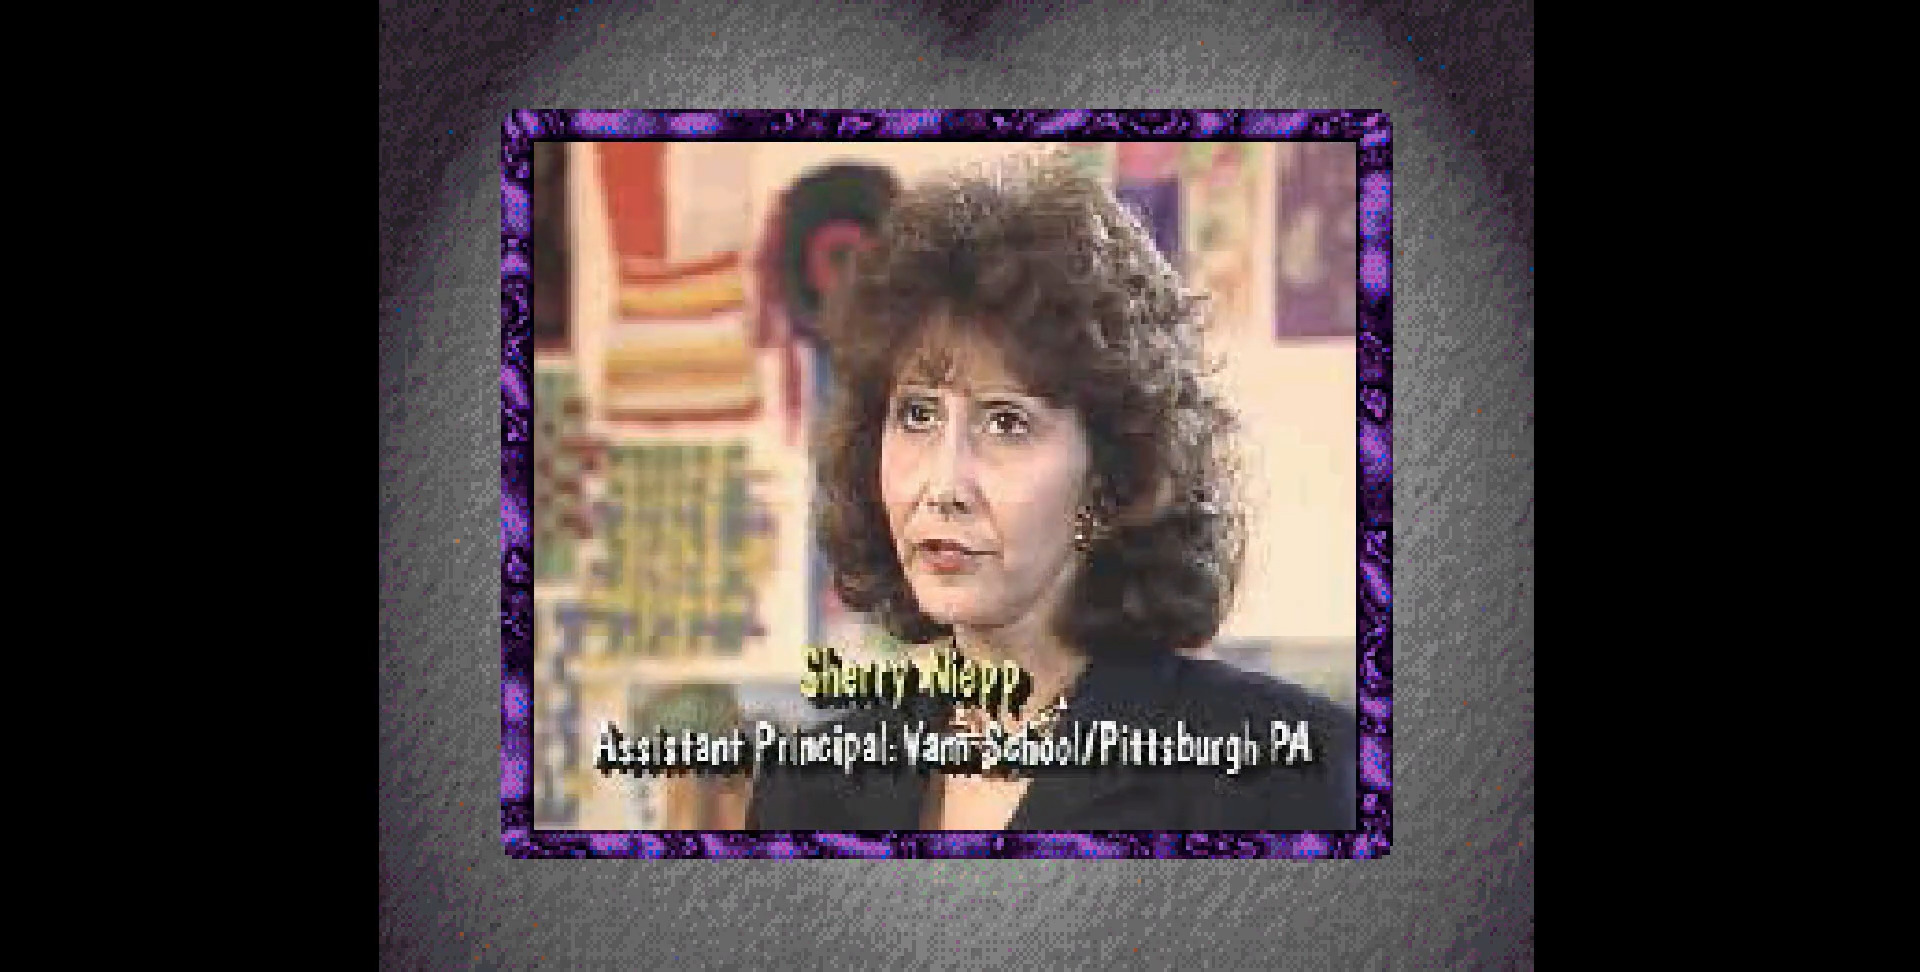
\includegraphics[width=\linewidth]{Games/EveryChildCanSucceed/Images/EveryChildCanSucceedScreenshot1.jpg}
        \caption{Every Child Can Succeed - Screenshot 1}
    \end{subfigure}
    \begin{subfigure}{0.45\textwidth}
        \centering
        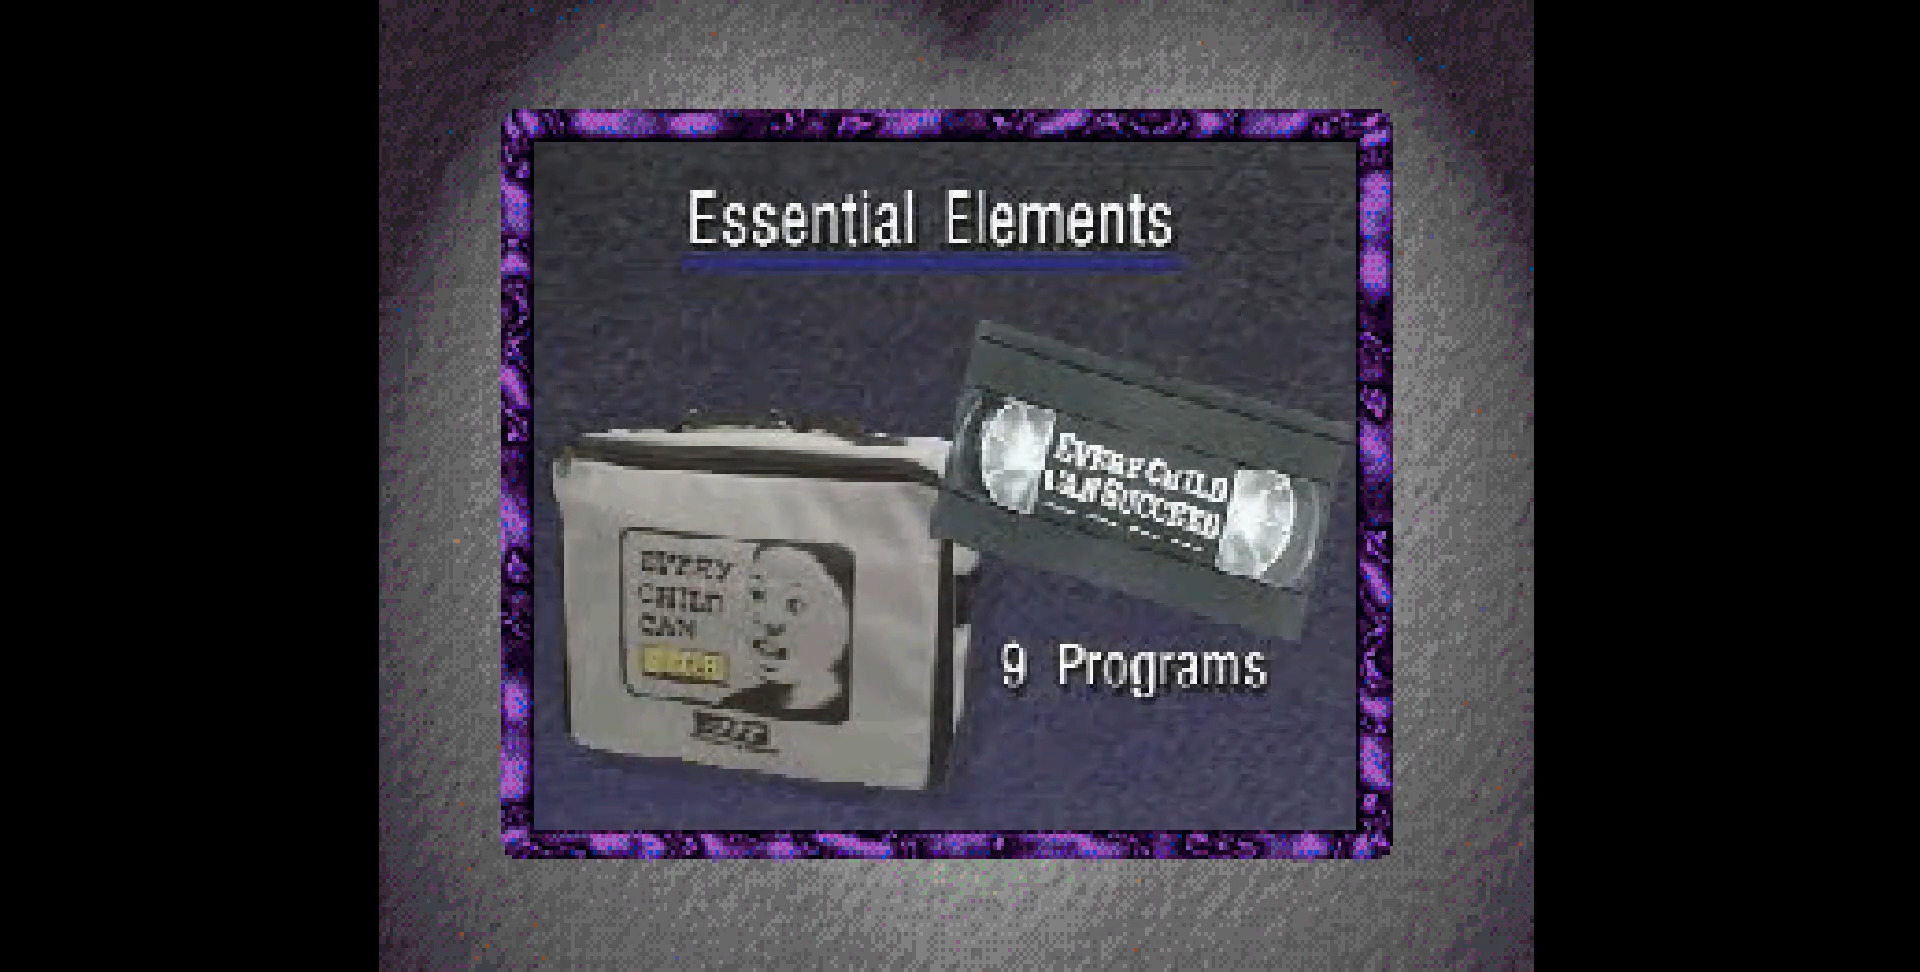
\includegraphics[width=\linewidth]{Games/EveryChildCanSucceed/Images/EveryChildCanSucceedScreenshot2.jpg}
        \caption{Every Child Can Succeed - Screenshot 2}
    \end{subfigure}

    \begin{subfigure}{0.45\textwidth}
        \centering
        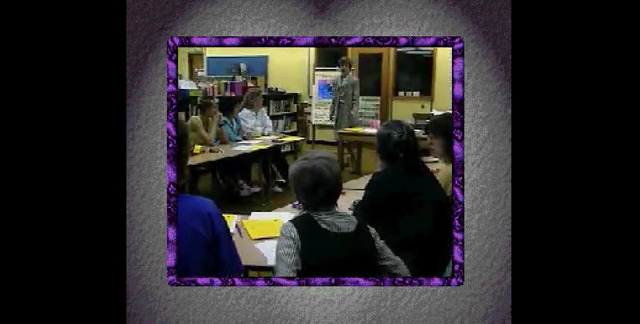
\includegraphics[width=\linewidth]{Games/EveryChildCanSucceed/Images/EveryChildCanSucceedScreenshot3.jpg}
        \caption{Every Child Can Succeed - Screenshot 3}
    \end{subfigure}
    \begin{subfigure}{0.45\textwidth}
        \centering
        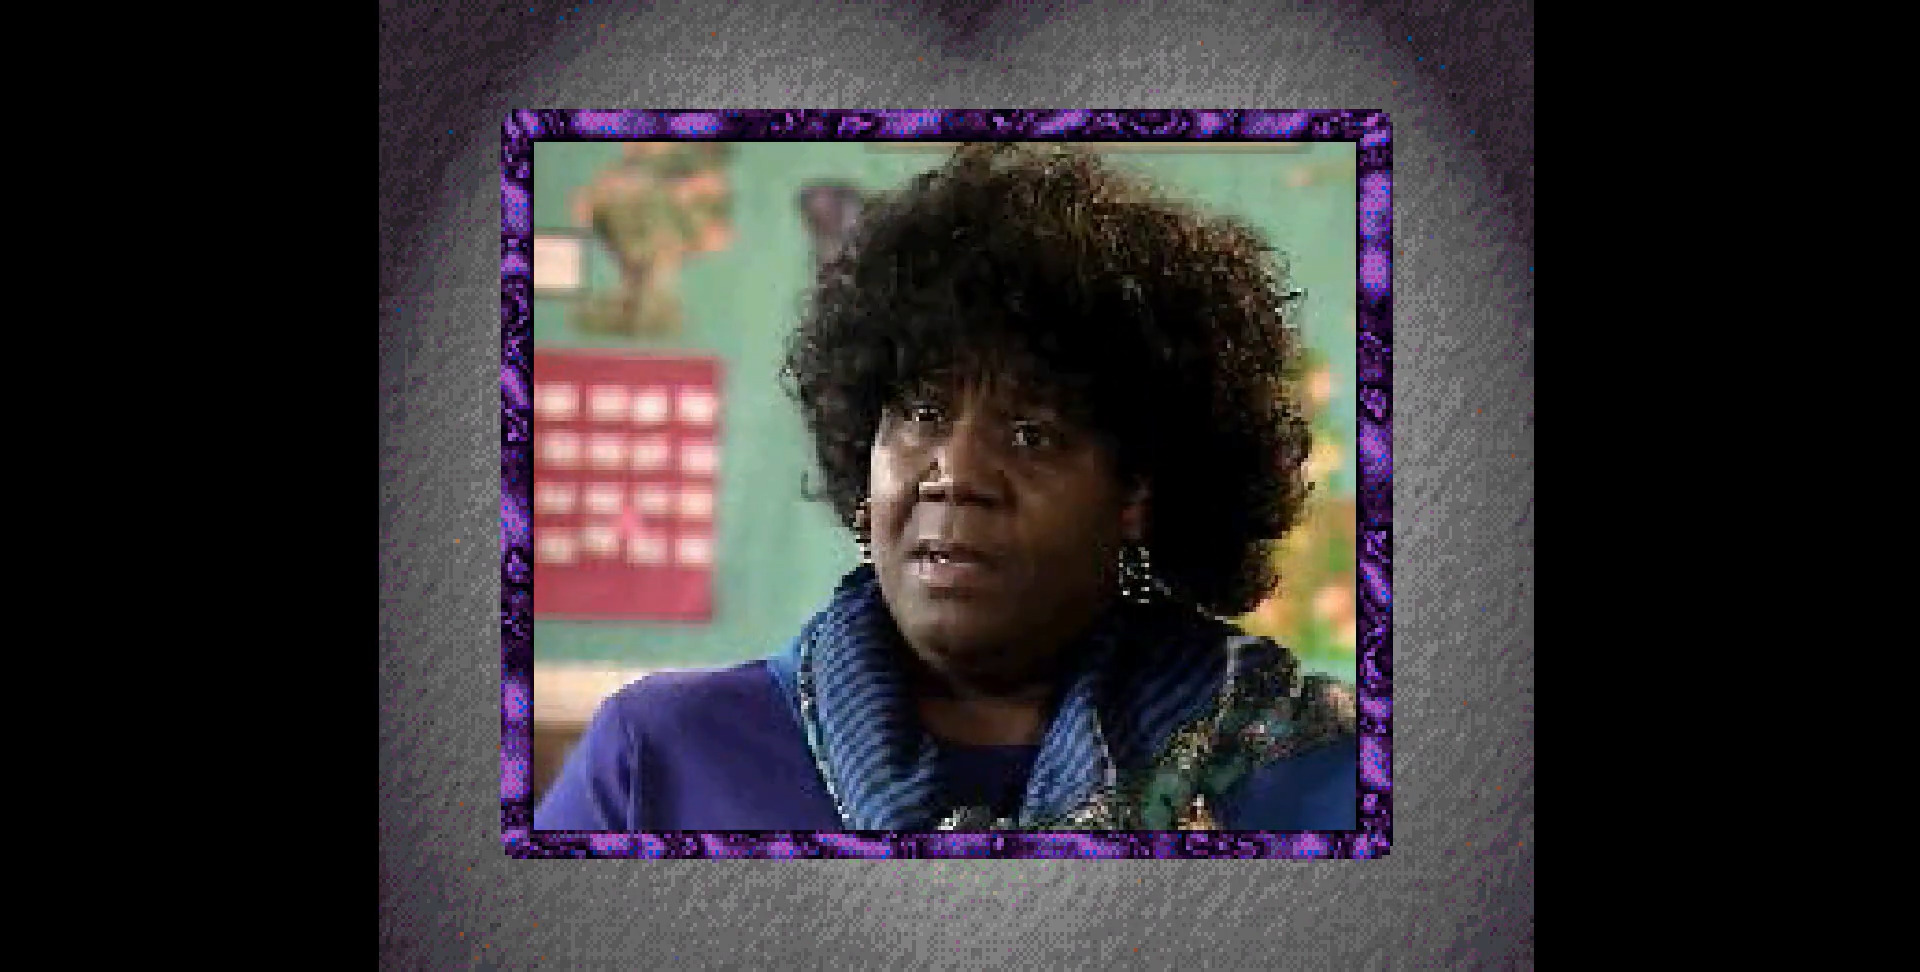
\includegraphics[width=\linewidth]{Games/EveryChildCanSucceed/Images/EveryChildCanSucceedScreenshot4.jpg}
        \caption{Every Child Can Succeed - Screenshot 4}
    \end{subfigure}
    \begin{subfigure}{0.45\textwidth}
        \centering
        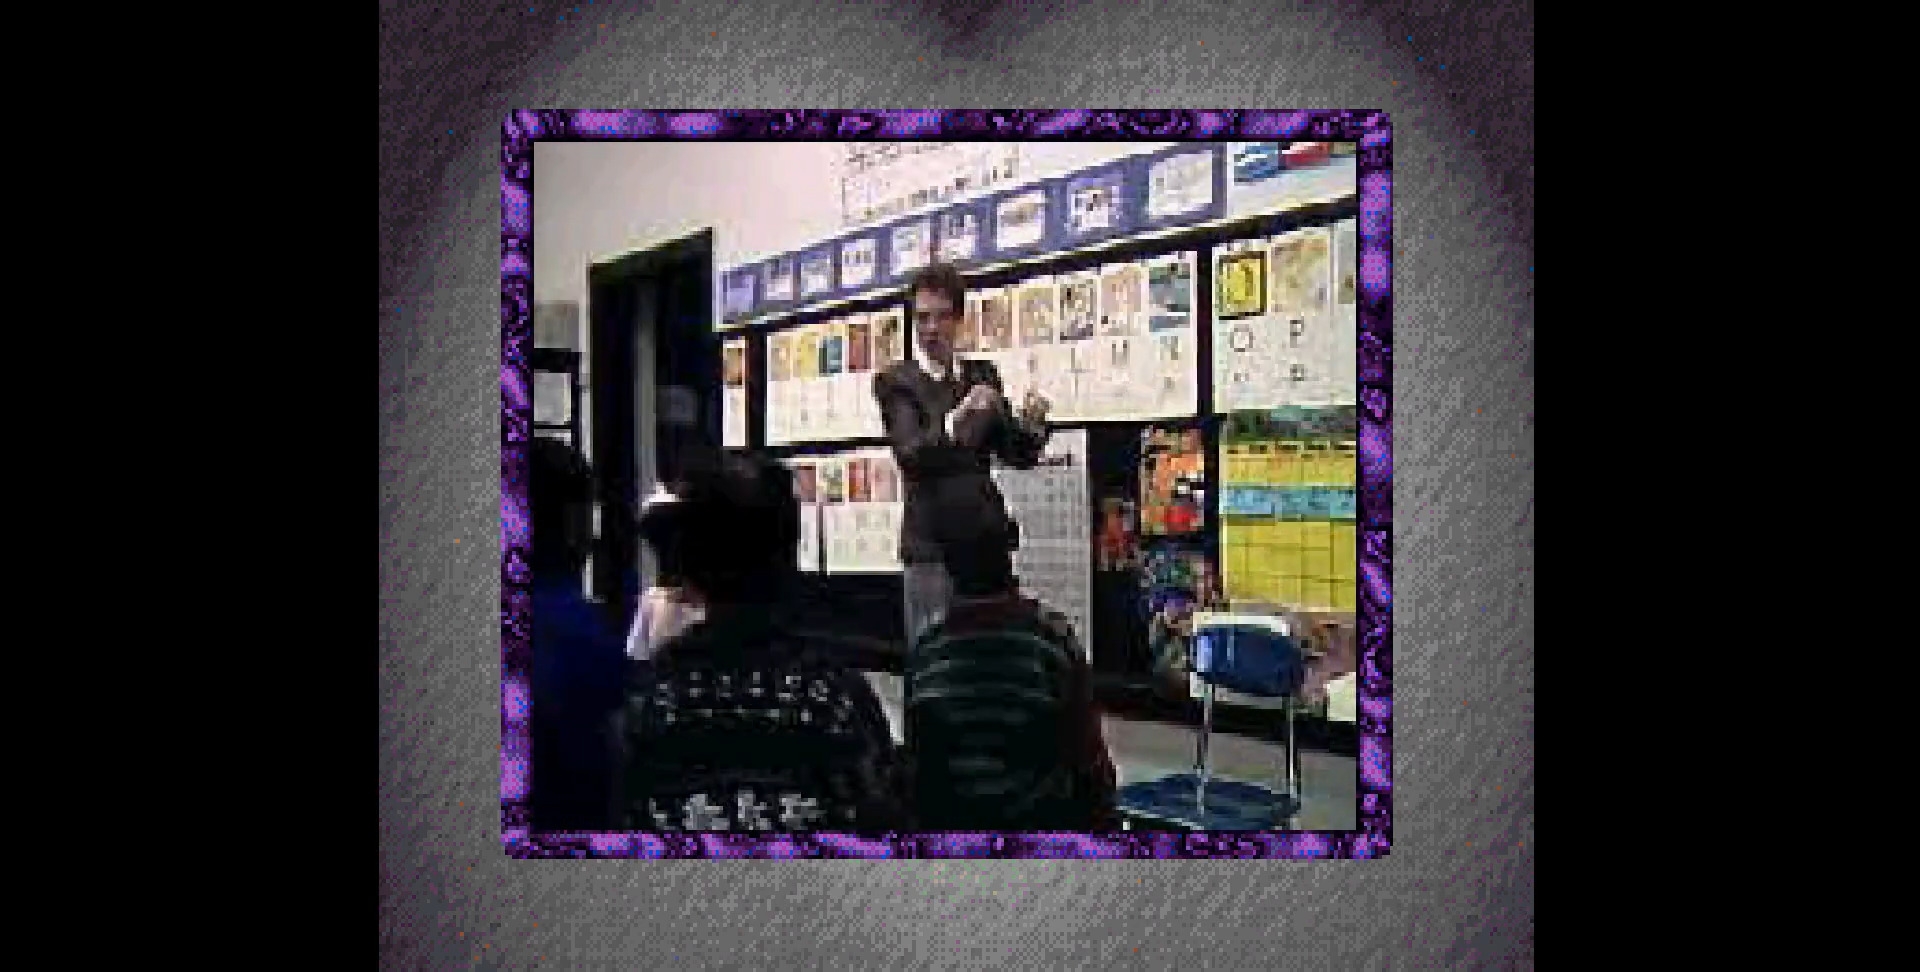
\includegraphics[width=\linewidth]{Games/EveryChildCanSucceed/Images/EveryChildCanSucceedScreenshot5.jpg}
        \caption{Every Child Can Succeed - Screenshot 5}
    \end{subfigure}
    \begin{subfigure}{0.45\textwidth}
        \centering
        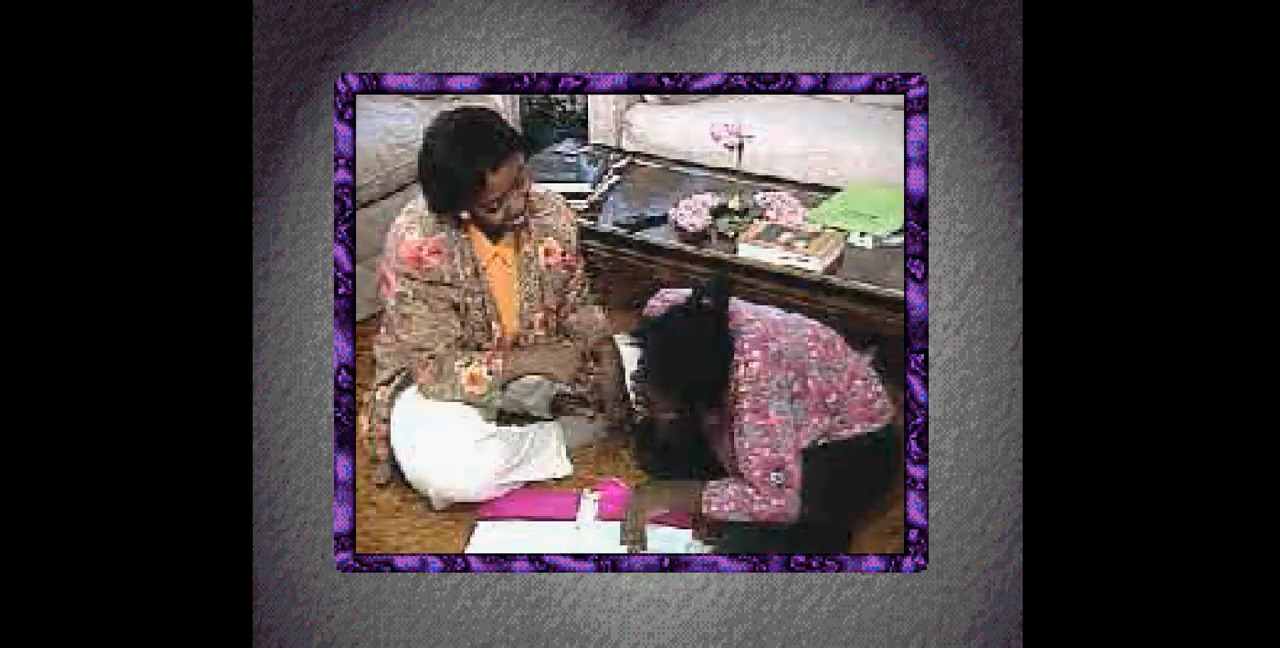
\includegraphics[width=\linewidth]{Games/EveryChildCanSucceed/Images/EveryChildCanSucceedScreenshot6.jpg}
        \caption{Every Child Can Succeed - Screenshot 6}
    \end{subfigure}
    \caption{Screenshots from the Every Child Can Succeed Series}
\end{figure}
